\chapter{Конструкторская часть}

В данной части будут представлены схемы последовательного и параллельного алгоритма, реализации функции генерации участка изображения и реализации рабочего потока.

\section{Разработка алгоритмов}
Для обоих алгоритмов использовалась одна и та же функция для генерации участка изображения. В последовательном алгоритме она вызывается один раз для всего изображения, а в параллельном для каждой области.

На рисунке~\ref{fig:risunok_1} изображена схема реализации последовательного алгоритма.
\begin{figure}[H]
	\centering
	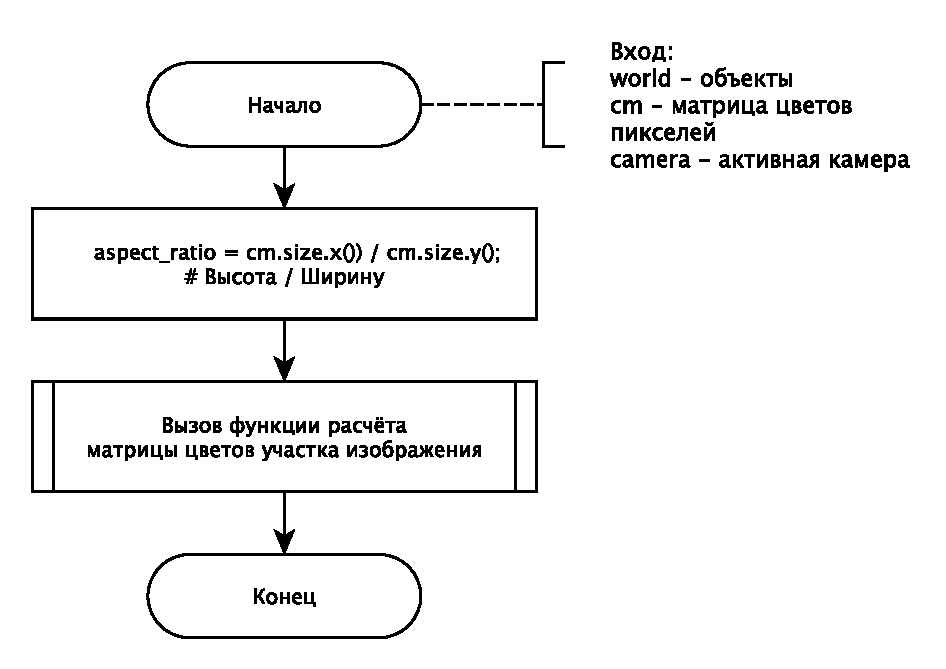
\includegraphics[width=0.7\textwidth]{images/AA2_1.pdf}
	\caption{Схема реализации последовательного алгоритма}
	\label{fig:risunok_1}
\end{figure}

На рисунке~\ref{fig:risunok_2} изображена схема реализации алгоритма генерации участка изображения.
\begin{figure}[H]
	\centering
	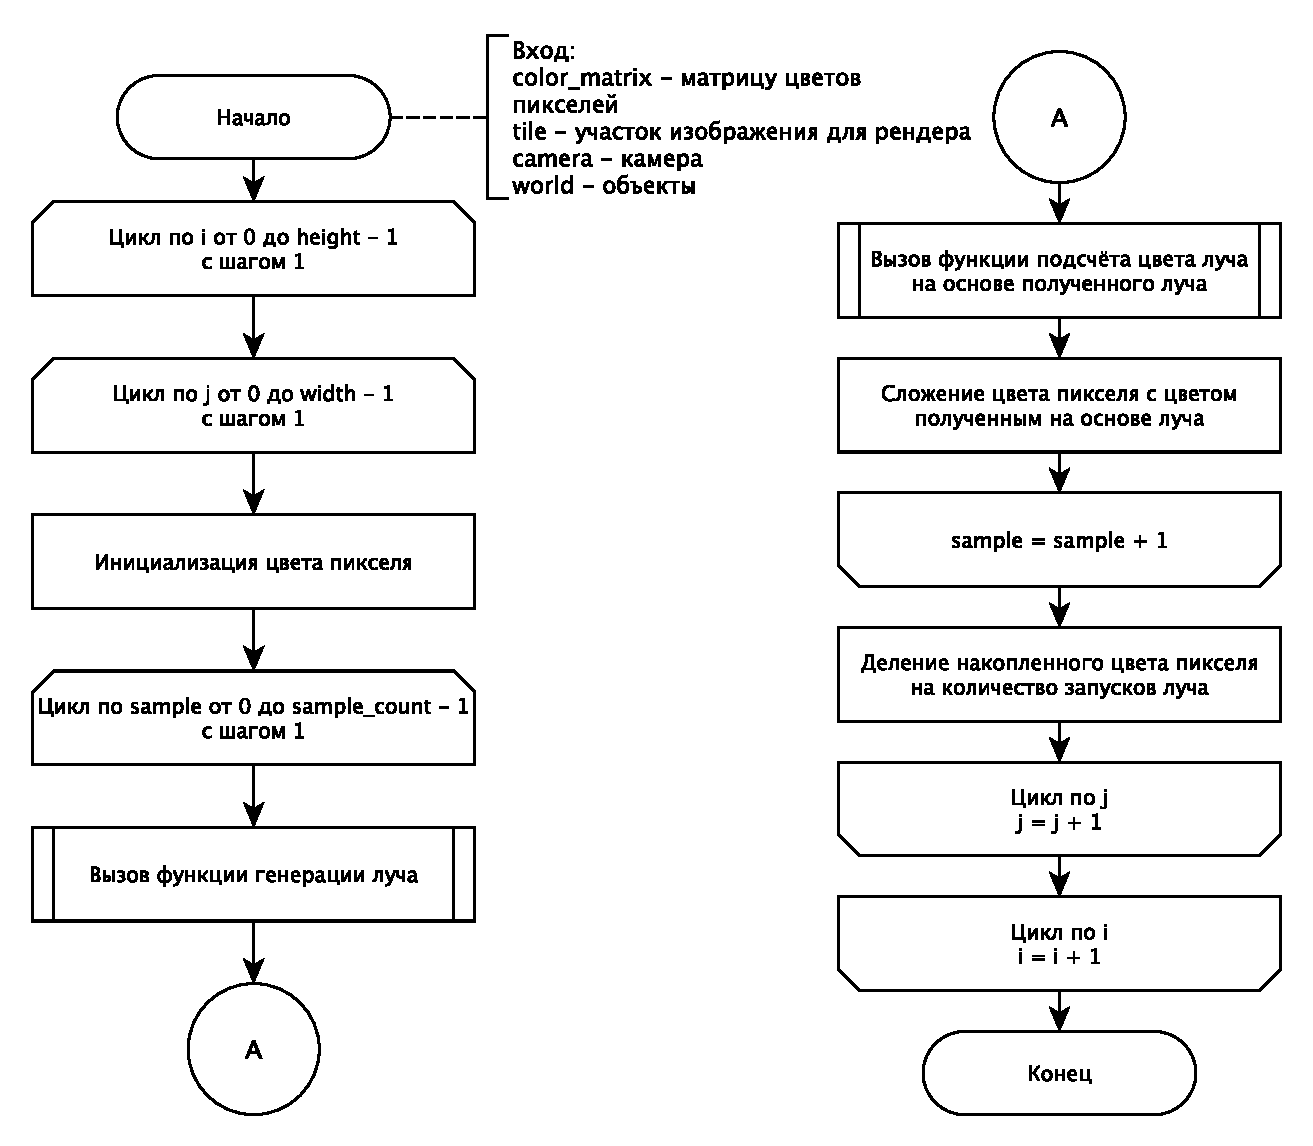
\includegraphics[width=1\textwidth]{images/AA2_2.pdf}
	\caption{Схема реализации алгоритма генерации участка изображения}
	\label{fig:risunok_2}
\end{figure}

На рисунках~\ref{fig:risunok_3}~и~\ref{fig:risunok_4}  изображена схема реализации главного потока параллельного алгоритма.
\begin{figure}[H]
	\centering
	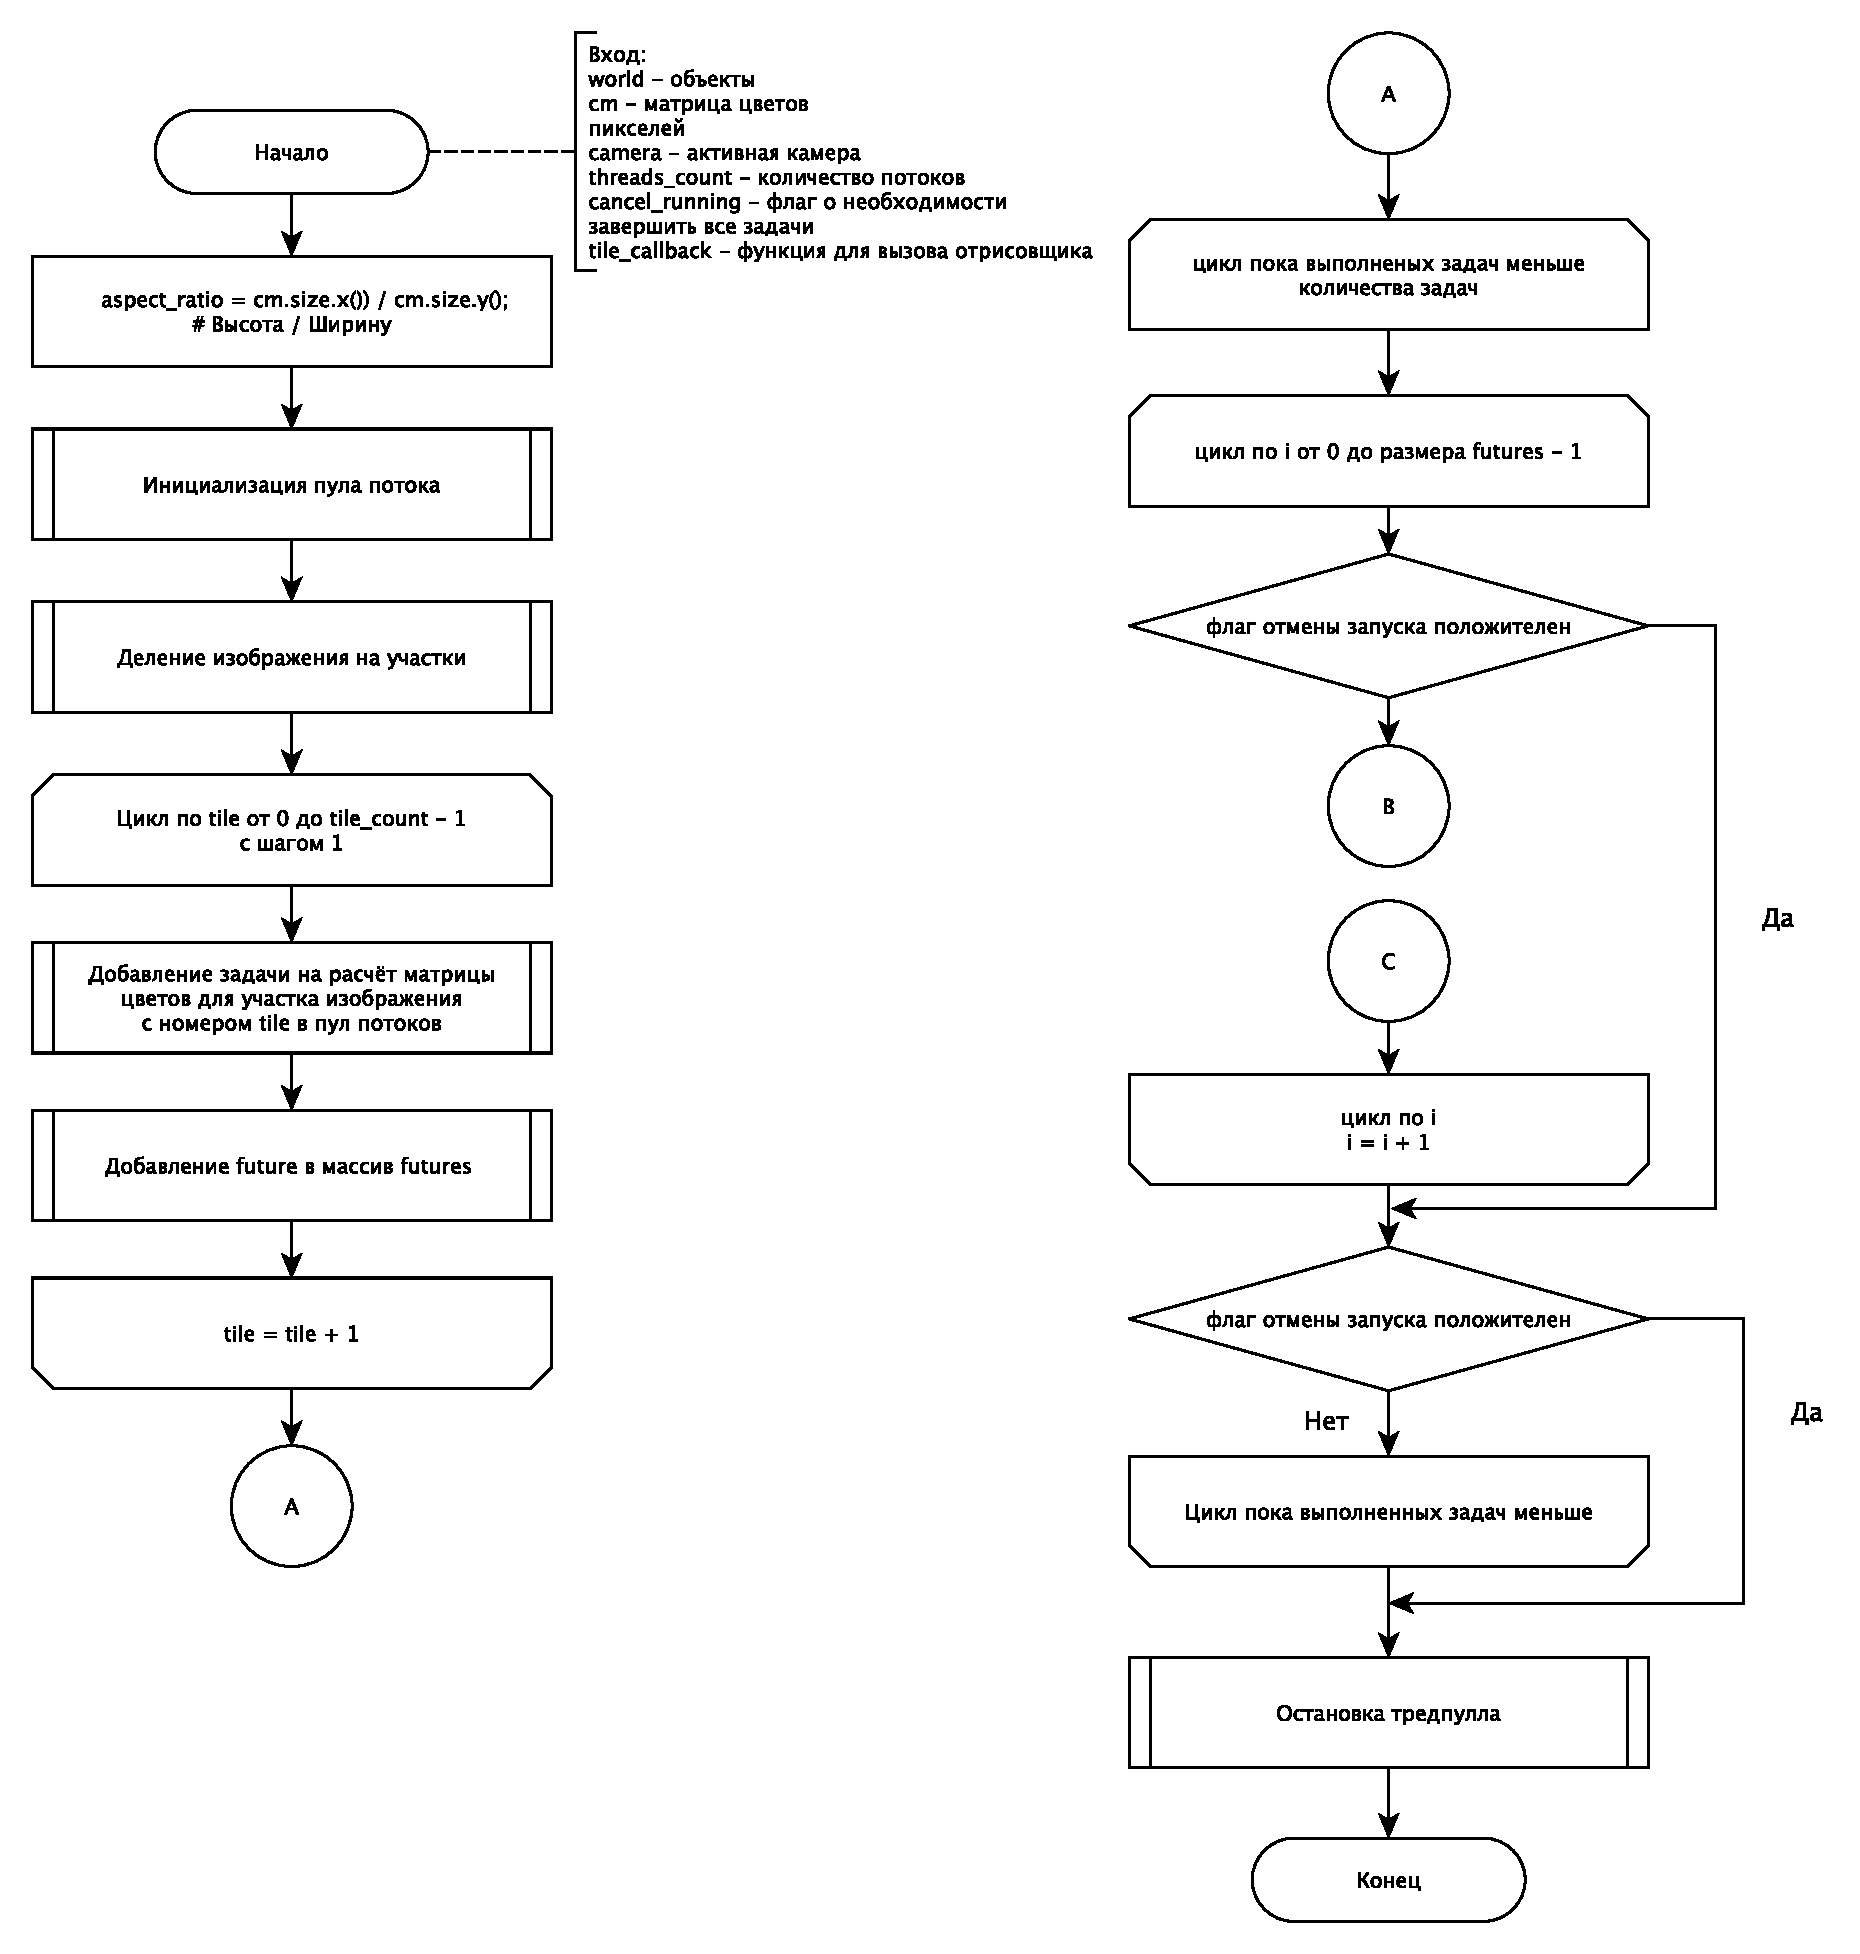
\includegraphics[width=1\textwidth]{images/AA2_3.pdf}
	\caption{Схема реализации главного потока параллельного алгоритма -- ч. 1}
	\label{fig:risunok_3}
\end{figure}

\begin{figure}[H]
	\centering
	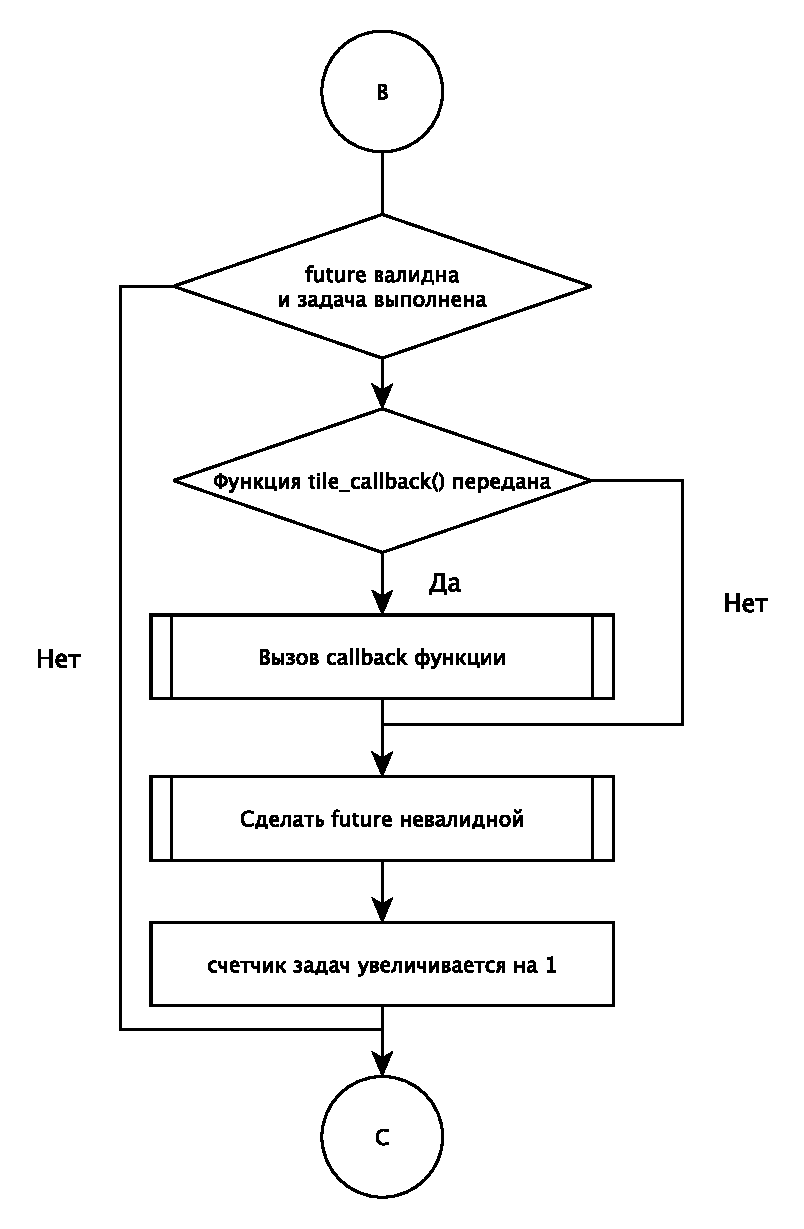
\includegraphics[width=0.7\textwidth]{images/AA2_4.pdf}
	\caption{Схема реализации главного потока параллельного алгоритма -- ч. 2}
	\label{fig:risunok_4}
\end{figure}

\section{Разработка средства для параллельного выполнения программы}

Для реализации моего варианта была разработана собственная реализация пула потоков. Поскольку изображение разбивается на большое количество небольших областей, создание отдельного потока для каждой задачи привело бы к значительным накладным расходам: выделение стека, инициализация в ядре ОС и последующее переключение контекста. Чтобы избежать этих издержек, все задачи помещаются в общую очередь, а фиксированное число рабочих потоков последовательно извлекают и выполняют их по мере освобождения. Такой подход минимизирует затраты на создание потоков и обеспечивает эффективную утилизацию ресурсов.

На рисунке~\ref{fig:risunok_5} изображена схема реализации рабочего потока пула потоков.
\begin{figure}[H]
	\centering
	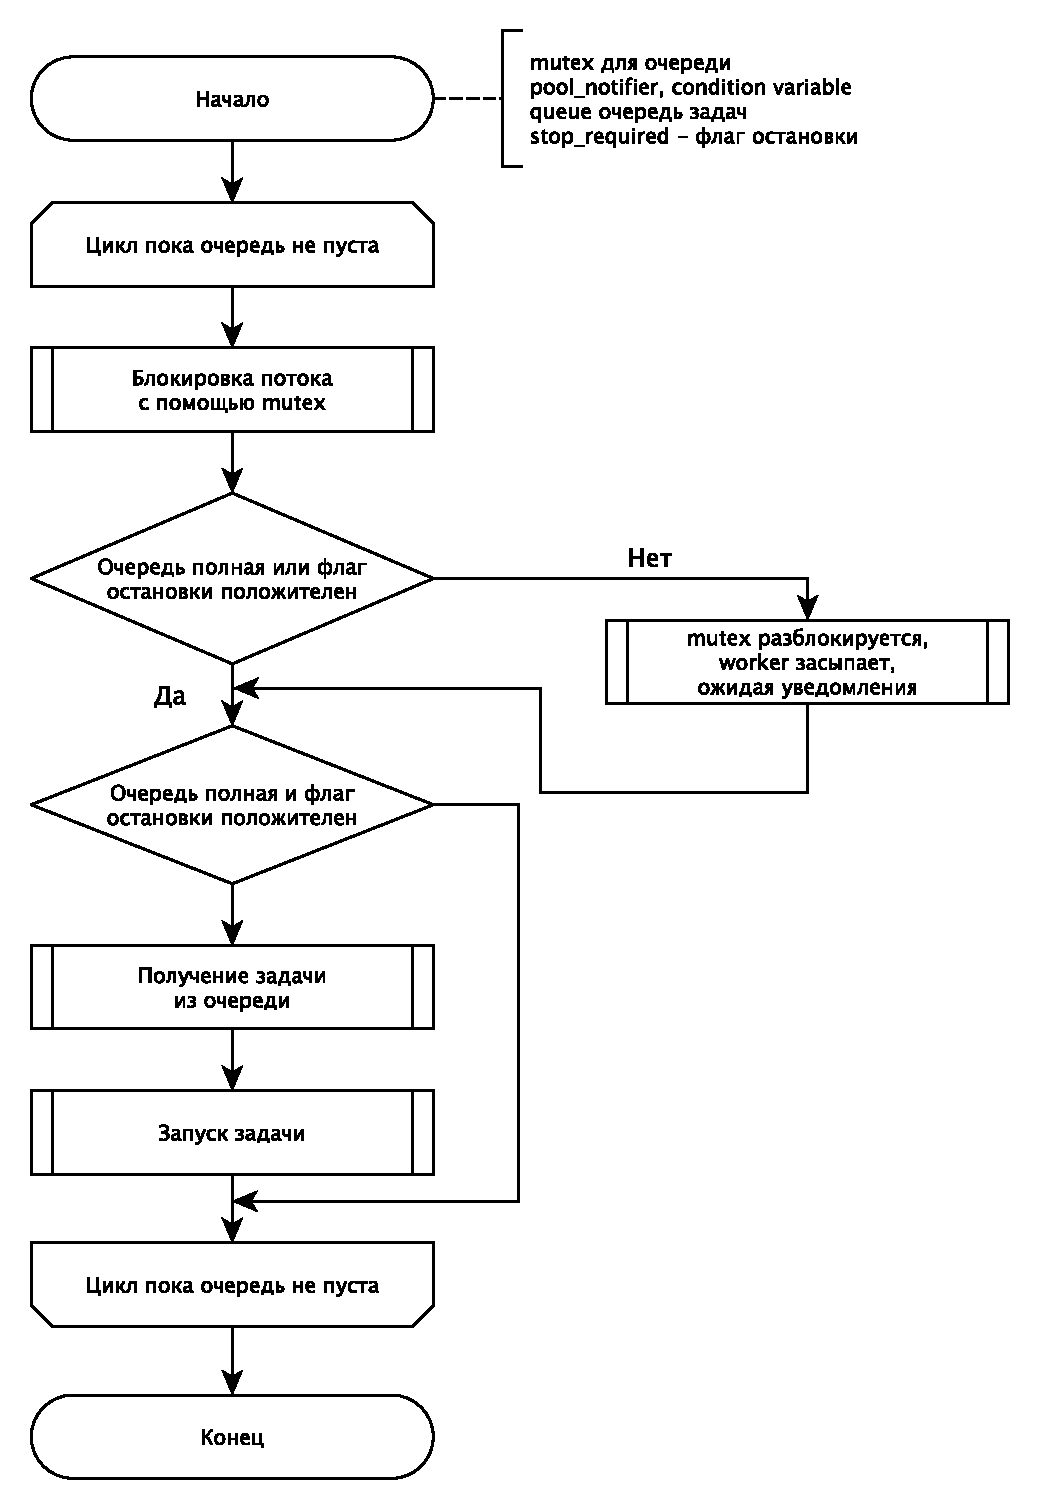
\includegraphics[width=0.7\textwidth]{images/AA2_5.pdf}
	\caption{Схема реализации рабочего потока пула потоков}
	\label{fig:risunok_5}
\end{figure}

\section{Генерация изображения по областям}

Для улучшения пользовательского опыта было приятно решение открывать интерфейс сразу, а не после генерации всего изображения. При создании изображения, области выводятся в интерфейс сразу после окончания их генерации. Чтобы не блокировать основной поток с интерфейсом, необходимо разделить программу на 2 потока:
\begin{itemize}
	\item поток для работы с графическим фреймворком;
	\item поток для генерации изображения.
\end{itemize}

\section{Типы данных}

В качестве примитивов синхронизации были выбраны $std::mutex$~\cite[c.~1784--1791]{lit2} и~$std::condition\_variable$~\cite[с.~1583--1690]{lit2}. Для возможности получения результата задачи использовался $std::future$~\cite[с.~1595--1602]{lit2}.

Данные о матрице цветов пикселей хранятся в классе $ColorMatrix$, 
представляющий собой std::vector. Количество потоков задаётся типом данных $size\_t$. Флаг отмены задаётся типом $bool$, а callback функция с помощью класса $std::function<void>$

Для запуска генерации в отдельном потоке и обхода блокировки графического потока, использовался метод $run()$ из класса $QtConcurrent$~\cite{QtConcurrent}.

\section*{Вывод}

В данной части были представлены схемы последовательного и параллельного алгоритма, реализации функции генерации участка изображения и реализации рабочего потока.